\documentclass{ximera}

\title{General Syllabus}
\begin{document}
\begin{abstract}
This is the syllabus for the course with everything but grading and the calendar
\end{abstract}
\maketitle

This is MAC1140 "Precalculus Algebra". The goal of this course is to provide the mechanical and conceptual tools necessary to continue on to MAC2311 "Calculus One" except for trigonometry, which can be taken separately by taking MAC1114 "Trigonometry". Alternatively one can take the accelerate combined Precalculus algebra and trigonometry class MAC1147.

A minimum grade of C (not C-) in MAC 1140 satisfies four credits of the university General Education Math requirement.%

\subsection*{Prerequisites}
\begin{center}
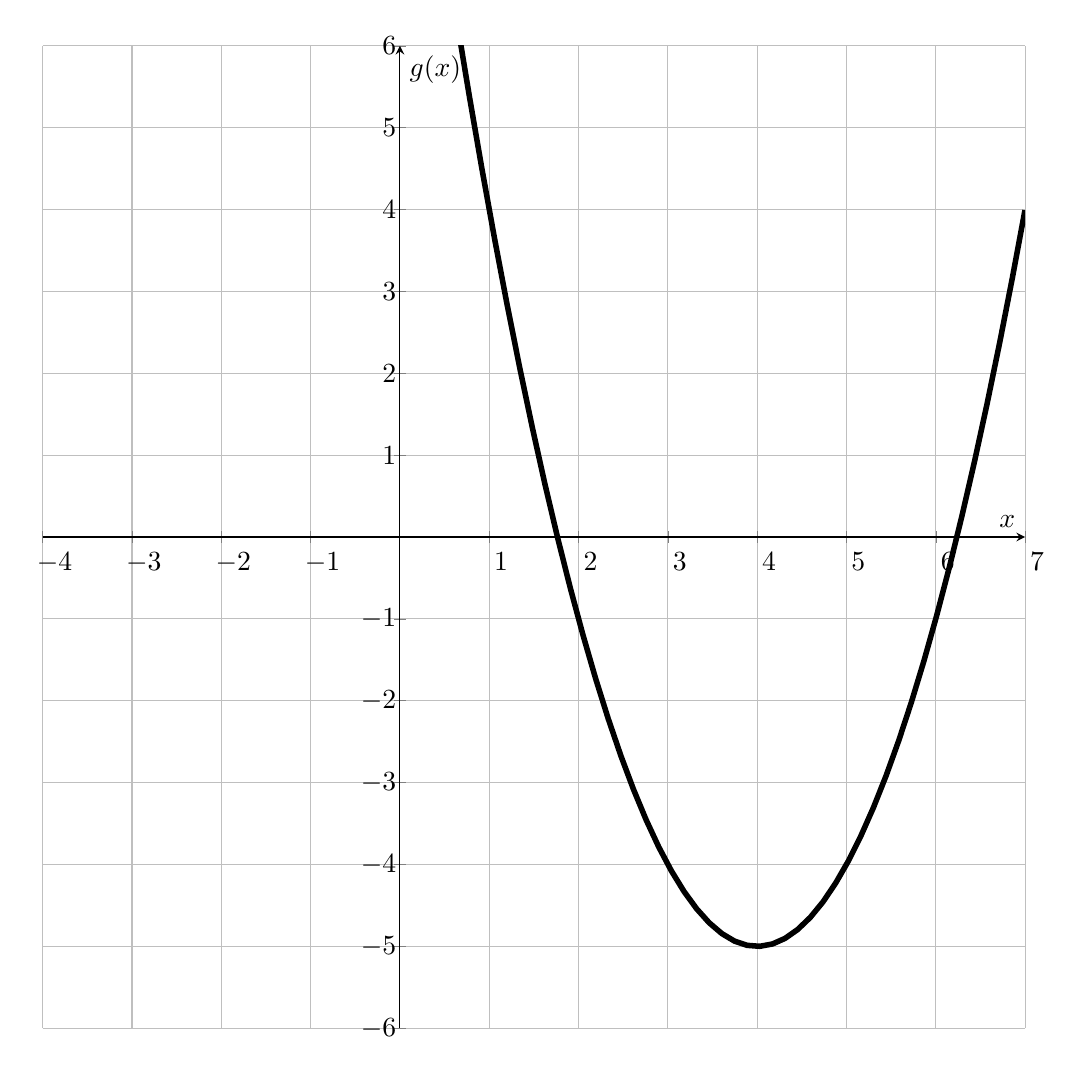
\begin{tikzpicture}
\begin{axis}
[
width=400,
height=400,
xmin=-4,
xmax=7,
ymin=-6,
ymax=6,
grid=both,
minor x tick num=0,
minor y tick num=0,
axis lines = middle,
ticklabel style = {xshift=1ex},
xlabel = $x$,
ylabel = $g(x)$
]
\addplot[domain=-7:7,samples=100, line width=2 pt]{(x-4)^2-5};
\end{axis}
\end{tikzpicture}
\end{center}


\subsubsection*{Course Materials}
%%%%%  Textbooks and things
    There  are  no  required  materials for this course; specifically there is no required textbook, clicker, or online homework code that you must purchase for  this  course. % This is a general statement for any course I teach, ideally.
    
    In this course we will utilize a free online homework system known as Xronos. This work is supported by the Office of the Provost and the College of Liberal Arts and Sciences.  The platform is accessible through the Canvas site.  More details will be given in class.


\subsubsection*{Online Resources}
%%%%%  Canvas, Xronos, WebAssign....
    E-learning Canvas, a UF course management system, is located at \url{elearning.ufl.edu}.  Use your Gatorlink username and password to login.  All course information including your grade, course homepage, syllabus, lecture videos,  office  hours,  test locations,  mail tool,  discussion forum,  free help information,  etc. can be accessed from this site.  \textbf{You are responsible for verifying that your grades are accurate.  There is no grade dispute at the end of the semester} (see below for the One Week Policy).

\subsubsection*{One Week Policy}

    Please be aware of the \textbf{One Week Policy}: Once you receive a graded paper back, you have \textbf{one week} to contest the grade and initiate any grade disputes. Once this one week passes, \textbf{there are no further disputes}. In particular, once the end of the semester nears, you \textit{cannot} start disputing, say, grades from the first week or two. 


\subsubsection*{Calculators}
    A graphing calculator and Wolframalpha are useful as study and learning tools when used appropriately, \textbf{but they are not essential.}  I also recommend the online graphing calculator Desmos (\url{www.desmos.com}), and the app GeoGebra (\url{www.geogebra.org}) to help you as you learn the material, but mathematics is a collection of ideas that are not mastered through calculator skills.  \textbf{No calculators are allowed on quizzes or exams.}

\subsubsection*{Lectures}

This course serves a number of goals. 
\begin{itemize}
    \item First and foremost this course is intended to get studens prepared for the UF calculus sequence. The calculus sequence is \textit{considerably} more rigorous and difficult than high school or advanced placement (AP) type courses, and the precalculus courses are similarly much more difficult in preparation of this. In particular, even students that routinely have gotten A's in their math courses in high school will likely find this course quite challenging.
    \item This course also aims to get everyone on the same mathematical level in terms of notation, communication, and terminology before students move forward. As such there will inevitably be times when you will find the content boring or otherwise elementary. This is because not everyone will be familiar with any given aspect, which means we must cover everything to some extent. However, due to the quantity of material that we need to cover from this, each of these excursions will be only a brief overview.
    \item In this course we also aim to instill the basics of mathematical reasoning. This means teaching how to problem solve when presented with content that is otherwise unfamiliar. Importantly this means that \textit{you should expect to be confronted with problems that you have not seen before}. If you have always had problems that are variations of problems that have been demonstrated for you already, then your teachers have done you a grave disservice. 
    \item \textbf{Expect to have to reason and think on the fly during exams, quizzes, and homework.} You will almost certainly see questions on your assessments that are unfamiliar. Remember that part of lecture is teaching you \textbf{how to recognize aspects of a problem to see what techniques to use}.
    \item Finally, remember that math, by it's nature, is cumulative. If an exam has listed content that will be tested, that means that the content is the \textit{focus} of the exam, but \textit{not the only skills necessary for the exam}. Clearly we will not list on every exam things like `addition' or `multiplication' as exam topics. Similarly, most of the content that we will cover in this class, by it's nature, will be used in future content of this same course. Thus you should consider all exams as ``cumulative" with the listed content for the exam being the primary \textit{focus} of the exam.
\end{itemize}

\subsubsection*{Incomplete Policy}
    A grade of I (incomplete) will be considered only if you meet the Math Department criteria which is found at \url{http://www.math.ufl.edu}.  If you meet the criteria you must see the instructor before the beginning of finals week to be considered for an I.  A grade of I only allows you to make up your incomplete work. You cannot redo any previously completed work.


\subsubsection*{Online Course Evaluation}
    Students are expected to provide feedback on the quality of instruction in this course by completing online evaluations at \url{https://evaluations.ufl.edu}. Evaluations are typically open during the last two or three weeks of the semester, but students will be given specific times when they are open. Summary results of these assessments are available to students at \url{https://evaluations.ufl.edu/results/}.

\subsubsection*{Advising and Help}  %%% YOU MAY AMMEND THIS DEPENDING ON THE COURSE
    For all concerns with MAC1140, please talk to your TA!  Office hours will be posted and are regular times when they are available to answer questions, discuss grades, advise students on future classes, or help students in any available way. You do \textbf{not} need an appointment to visit during office hours. If you need to meet outside of office hours, please contact your TA for an appointment. \\


    \noindent In addition, there are several other free resources available to you:
    \begin{itemize}
        \item The Teaching Center Math Lab, located at SE Broward Hall, offers free informal tutoring. You may want to attend different hours to find the tutors with whom you feel most comfortable.  Also the Little 215 Tutoring Center provides free tutoring for courses up to Calculus 1.  Go to \url{http://www.teachingcenter.ufl.edu} to find their hours. You can also request free one-on-one tutoring.
    
        \item A list of qualified tutors for hire is available at \url{http://www.math.ufl.edu}.
    \end{itemize}

\subsubsection*{Honor Code}
    All students are required to abide by the Academic Honesty Guidelines which have been accepted by the University. The academic community of students and faculty at the University of Florida strives to develop, sustain and protect an environment of honesty, trust and respect. Students are expected to pursue knowledge with integrity.\\

    \noindent Violations of the Academic Honesty Guidelines shall result in judicial action and a student being subject to the sanctions in paragraph XIV of the Student Code of Conduct. The conduct set forth hereinafter constitutes a violation of the Academic Honesty Guidelines (University of Florida Rule 6C1-4.017).  You may find the Student Honor Code and read more about student rights and responsibilities concerning academic honesty at the link \url{www.dso.ufl.edu/sccr/}.

\subsubsection*{Students with Disabilities}
    Students requesting classroom accommodation must first register with the Dean of Students Office \url{www.dso.ufl.edu/drc/}. The DOS will provide documentation to the student who must then provide this documentation to the course instructor. Any accommodations must be submitted \underline{as soon as possible}.  If a student does not supply the appropriate documentation in a timely fashion, the instructor may not be able to accommodate the student in a timely manner.     
    


\end{document}
